\documentclass[10.5 pt, conference]{IEEEtran}       
\overrideIEEEmargins
\usepackage[a4paper,left=1.4cm,right=1.4cm,top=1.5cm,bottom=2cm,showframe=false]{geometry}
\usepackage{graphicx}
\usepackage{siunitx}
\usepackage{url}
\usepackage{tabularx}
\usepackage{caption}
\usepackage{booktabs}
\usepackage{tabularx}
\usepackage{gensymb}
\usepackage[noadjust]{cite}
\usepackage{filecontents}
\usepackage{float}
\usepackage{hyperref}
\usepackage[table,xcdraw]{xcolor}
\usepackage{amsmath}
\usepackage{algorithm}
\usepackage[noend]{algpseudocode}
\pagenumbering{arabic}
\usepackage{setspace}
%\onehalfspacing
%\doublespacing
\renewcommand{\IEEEbibitemsep}{0pt plus 0.5pt}
\makeatletter
\IEEEtriggercmd{\reset@font\normalfont\fontsize{7.9pt}{8.40pt}\selectfont}
\makeatother
\IEEEtriggeratref{1}

%\usepackage{subcaption}
%\usepackage{amssymb}
\newcommand{\inlinemaketitle}{{\let\newpage\relax\maketitle}}
\makeatletter
\def\@maketitle{%
  \newpage
%  \null% DELETED
  \vskip 1.5em
  \begin{center}%
  \let \footnote \thanks
    {\LARGE \@title \par}%
    \vskip 1.0em%
    {\small
      \lineskip .2em%
      \begin{tabular}[t]{c}%
        \@author
      \end{tabular}\par}%
    \vskip 1.5em%      \centering
		%\line(1,0){50}
  \end{center}%
  \par
  \vskip 1em}
\makeatother

\title{
\includegraphics[width=19.0cm]{Report_Title_cover.png}\vspace*{-0.2cm}}
\author{ \\ Christopher Maree (1101946) \text{    } Iordan Tchaparov (1068874)	\text{    }	 Laura West (1084327) \text{    }Kavilan Nair (1076342) }

%%%%%%%%%%%%%%%%%%%%%%%%%%%%%%%%%%%%%%%%%%%%%%%%%%%%%%%%%%%%%%%%%%%%%%%%%%%%%%%%
\begin{document}
\maketitle
\thispagestyle{empty}
\pagestyle{plain}
%\doublespacing
%%%%%%%%%%%%%%%%%%%%%%%%%%%%%%%%%%%%%%%%%%%%%%%%%%%%%%%%%%%%%%%%%%%%%%%%%%%%%%%%
\begin{abstract}
This paper presents and discusses three common relational database join algorithms, namely: Naive nested loop join, MapReduce reduce-side join and distributed hash-join using Message Passing Interface (MPI). Each implementation is discussed in detail and then benchmarked on a cluster testing platform. Results are critically analysed, drawing insight to relative performance metrics of each implementation. Benchmarks showed that a distributed implementation, created in MPI, proves to outperform the other two solutions. Faults of each method are discussed, along with possible future improvements. The Github repository can be found \href{https://github.com/data-intensive-computing-4020/Project}{here}.
\end{abstract}
%%%%%%%%%%%%%%%%%%%%%%%%%%%%%%%%%%%%%%%%%%%%%%%%%%%%%%%%%%%%%%%%%%%%%%%%%%%%%%%%
%\doublespacing
\thispagestyle{empty}
\pagestyle{plain}
\section{Introduction}
Databases are used in a myriad of modern technological applications, present in practically all systems involving the storage of data. A key concept in database design is normalisation of tables to protect data and to make the database more flexible by eliminating redundancy and inconsistent dependency. A resultant downside from normalisation is the need to perform relational joins between tables, a computationally expensive process. This paper presents and compares a selection of joining algorithms, implemented in Python. The primary point of comparison is between a distributed joining algorithm (implemented on a nine machine cluster over MPI) and a centralised version (using the Mapreduce Framework). A nested loop, naive variant was also implemented as a point of comparison. 

\section{Background}
\subsection{Distributed Computing}
High performance computer clusters are becoming more and more popular due to their scalability, affordability and reliability, as opposed to a centralized implementation \cite{Ceran2012}. Clusters enable far easier horizontal scaling as opposed to the vertical scaling of traditional high performance systems. By adding additional computer nodes to a cluster, more computational resources can be accessed without needing to change the underlying architecture. The benefits of cluster computing lend themselves well to Database Management Systems (DBMS) but due to data network limitations and configuration complexities, clusters are not very popular in this application \cite{Ceran2012}. With that said, due to advances in network technologies, interest in distributed databases systems is increasing. \\

A distributed join algorithm is proposed in this paper, through the use of Python’s Message Passing Interface (MPI4PY) library to facility the utilization of a cluster.

\subsection{Mapreduce Framework}
The MapReduce Framework was created by Google in 2004 to facilitate and simplify processing of massive datasets in parallel on clusters of computers \cite{McTaggart}. The framework was designed to operate on affordable consumer hardware, providing a low barrier to entry and offers high reliability through fault-tolerance. MapReduce can perform computations on both structured and unstructured data, enabling a wide selection of different algorithms to be applied through the framework. 

\subsection{Problem Overview}

\subsubsection{Problem Description}
Table join operations are one of the most important relational database queries. The join involves matching rows in two separate tables, based on a common column through a Cartesian product \cite{Mishra1992}. In most generic implementations, this involves the linking of two tables where the primary key of one table is stored in another table, as a foreign key. The use of primary and foreign keys is not a prerequisite, with a join merely needing a common column between the tables. \\

There are four main relational join types, namely: inner, outer(or full), left and right joins. The most common join type is an inner join, requiring that both tables have matching keys on which the join is performed. A graphical representation of these joins is shown in the Figure \ref{JoinTypes} below. An inner join can be represented mathematically by Equation (1).

\begin{equation}
R(A,B) \bowtie R(A,C) = R(A,B,C)
\end{equation}

Joins are inherently computationally expensive due to the iterative nature of the joining process \cite{Stephens2004}. There are a number of ways to improve the join speed such as the use of surrogate keys over natural keys (smaller required string length of comparison) , indexing the data, use of materialized views (effectively pre-computed joins) or table partitioning (split data set over multiple disks enabling higher I/O)\cite{Stephens2004}. Despite these possible improvements, joins still pose a computationally taxing task for a DBMS and as a result finding optimized joining algorithms is vital to managing large data sets.\\

A selection of different algorithms are available for performing table joins, with the most fundamental being nested loop, sort-merge and hash joins\cite{Chu}. The latter two joins, along with other variants of their implementation, are used extensively in modern DBMS architectures. Based on the given data set, it might be more beneficial to use a sort-merge join over a hash join, such as when the data is already ordered. If the data set is not ordered by the joining key then the hash join algorithm has been shown to outperform the sort-merge join on average and so have been chosen for this paper \cite{Albutiu}.

\begin{figure}[h!]
\centering
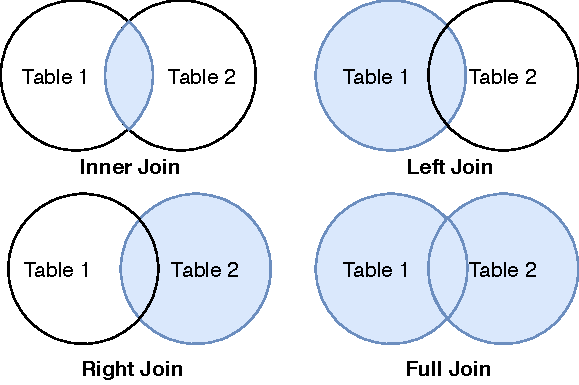
\includegraphics[width=\columnwidth]{JoinTypes.pdf}
\centering
\caption{Venn Diagram of Different Joins}
\label{JoinTypes}
\end{figure}

Joins are inherently computationally expensive due to the iterative nature of the joining process \cite{Stephens2004}. There are a number of ways to improve the join speed such as the use of surrogate keys over natural keys (smaller required string length of comparison) , indexing the data, use of materialized views (effectively pre-computed joins) or table partitioning (split data set over multiple disks enable higher I/O)\cite{Stephens2004}. Despite these possible improvements, joins still pose a computationally taxing task for a DBMS and as a result finding optimized joining algorithms is vital to managing large data sets.\\

A selection of different algorithms are available for performing table joins, with the most fundamental being nested loop, sort-merge and hash joins \cite{Mishra1992}. The latter two joins, along with other variants of implementation, are used extensively in modern DBMS. Based on the given data set, it might be more beneficial to use a sort-merge join over a hash join, such as when the data is already ordered. If the data set is not ordered by the joining key then the the hash join algorithm has been shown to outperform the sort-merge join on average and so have been chosen for this project\cite{Stephens2004}.\\

\subsection{Project Specifications}

\subsubsection{Assumptions and Constraints} 
The proposed algorithms must be run on the same system to ensure that the comparison is fair. The cluster provided is assumed to handle all underlying required network communications between nodes. The cluster is assumed to run consistently and that no other users will be using the machine or the network during the execution of benchmarks. 

\subsubsection{Success Criteria} 
The project will be deemed a success if all three implemented algorithms can correctly produce joined results. Moreover, architecture specific implementations, such as MPI, should scale with the resources allocated to them. Trend graphs should correspond to the expected shape as larger and larger tables are joined.

\subsection{Literature Contextualization} 
Due to the importance of joins in relational databases and their resultant extensive utilization, a wide selection of research has been conducted. Key papers and research pertaining to relevant join algorithms are outlined below.

\subsubsection{Comparison of Join Algorithms} 
\cite{Schuh2016,Helmer} discuss and compare a selection of different join algorithms, including but not limited to those implemented in this paper. These works discuss in-memory Equi-joins over a range of input sizes. They provide a valuable point of reference against which the results in this paper can be compared.

\subsubsection{MapReduce Join Algorithms} 
\cite{Bushan2007,Pigul,Blanas2010} provide a comparison of join algorithms, implemented using the MapReduce Framework. These papers outline tradeoffs in the utilisation of the framework and discuss its advantages and disadvantages over other implementations. All four provide extensive benchmarking and result analysis. \cite{Palla2009} discusses the use of MapReduce, specifically implemented on the Hadoop framework, providing a guide to extend the work presented in this paper to run on a Hadoop cluster.

\subsubsection{Distributed Join Algorithms} 
\cite{Barthels2017,Schneider1992,Yu1997} discuss the implementation of distributed join algorithms, providing valuable reference for the MPI implementation presented in this paper. \cite{Barthels2017} is of particular relevance wherein the authors present the implementation of distributed join algorithms, running on thousands of cores, implemented in C++, through the use of MPI. \cite{Barthels2017} presents a valuable discussion into advantages and disadvantages of distributed join algorithms as well as insight into architecture design.

\section{Implemented Algorithms}
Three different joining algorithms are implemented and compared, over a range of sample data. Each algorithm is implemented in Python and a high level overview of each algorithm is presented below.

\subsection{Language justification}
Python is the language of choice for big data processing due to its ease of use and rapid development time and hence is utilized \cite{Beck}. Additionally, Python has a low barrier to entry, enabling novice coders to quickly and easily pick up the language. This means that a multitude of implementations can be created, focusing heavily on the algorithmic implementations rather than being restricted due to language specific complexities, as is the case in C. \\

Python is an interpreted language unlike the compiled, low level languages such as C and Fortran. Subsequently, benchmark results produced will not be fairly comparable. The goal in picking Python is to implement a selection of different join algorithms and compare their performance, in the Python context.

\subsection{Input Standardisation and JSON}
All datasets read into and out of each algorithm are stored using JSON formatting to minimise the required string and csv parsing. This makes the verification of results easier as the output is already in a predefined data structure. Additionally, while the initial read in of information may be slower as a basic conversion from JSON to Python object is required, the lack of line by line parsing results in a quicker overall implementation \cite{TutorialsPoint2018}.

\subsection{Naive Join Algorithm}

The naive algorithm performs the join using two nested for loops. The outer loop iterates through the first table row-by-row. The inner loop is executed for each row of table one and iterates through the second table row-by-row. The key of table one is compared with that of table two. If the keys match, the rows of table one and table two are concatenated and appended to a final output table. Using the naive algorithm shows efficiency when table one is small and table two is pre-indexed and large \cite{Microsoft2012}. The naive algorithm is superior to merge joins and hash joins when small tables are used \cite{Microsoft2012}. However, inferior benchmarking results are yielded compared to merge joins and hash joins for large tables. This is demonstrated by its $O(n) = n^2$ time complexity. \\

The naive algorithm implementation is benchmarked by timing different sections of the code. The time to read the files from disc, the time to perform the join, the time to write to the output file and the total time for implementation are all measured. Benchmarks of disc I/O are computed as they give insight to whether the memory or the processing computation make up the majority of the implementation time.

\subsection{Hash Join Implementation Python Dictionary Utilization }
A hash join algorithm leverages the hash table data structure to improve the efficiency of performing equijoin operations on database tables. Hashtables contain worst case time complexity of $O(n) = n $ and $\theta(1)$ in the average case for insertion, deletion and search which make it suitable for use in Hash Join algorithms. Both the MapReduce and MPI implementations of the hash join algorithm, made use of Python’s dictionary data structure which inherently makes use of a hash table as the underlying mechanism and is subsequently used in the implementations \cite{TutorialsPoint2018}.

\subsection{Map Reduce}
A reduce-side join algorithm is implemented using MRJob, a Python MapReduce library. This algorithm performs the joining operation in the reducer phase of the MapReduce as opposed to performing it in the mapper phase as done by map-side join algorithms. The map-side join algorithm needs small tables as it stores them in memory, indicating poor performance as the size of tables scales \cite{Priyanka2013}. The reduce-side join algorithm can be used on any data size without restrictions and is therefore implemented in this paper \cite{Mohamed2015}.\\

The implemented reduce-side join algorithm makes use of one mapper phase and two reducer phases. In the mapper phase, all the input records are read in as an iterable array. During each iteration, an intermediate key-value pair is generated for each record. The key is the primary key in one table and the foreign key in another table, this being determined by the selected column to join on. The value is the entire record for that instance of iteration. An identifier for records’ table of origin is added into the value of the key-value pairs and it is used to deal with duplicate records. It ensures that all matching keys allow the records to be correctly joined as many times as they appear in the table. The reducer phase then takes these key-value pairs, sorting and grouping the values together based on matching keys. This grouping is the joining of the records. The second reducer phase serves only to group all the joined records to allow a usable output format.\\ 

\begin{figure}[h!]
\centering
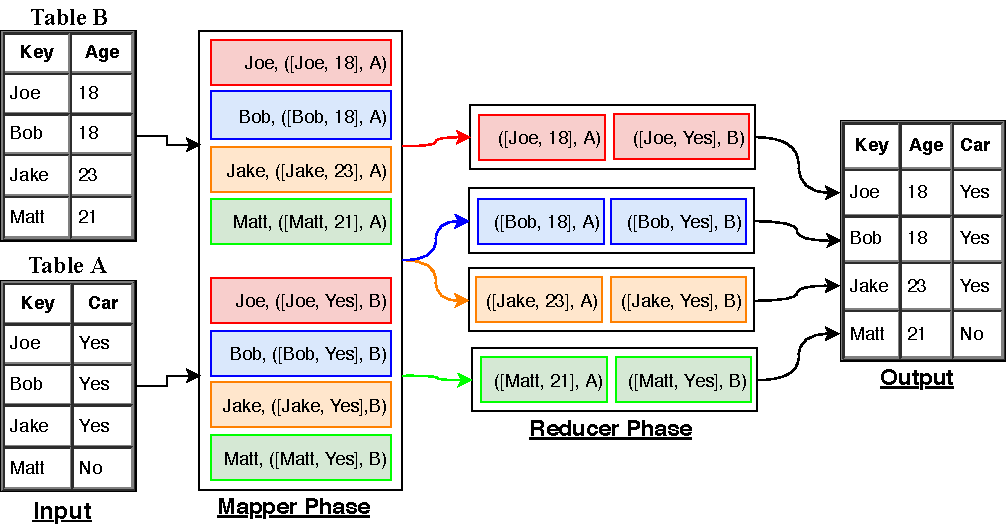
\includegraphics[width=\columnwidth]{MRDiagram.pdf}
\centering
\caption{Illustration of Reduce-Side Join Algorithm}
\label{MRJoin}
\end{figure}

The main benefit of MapReduce is that it simplifies data processing by distribution on multiple nodes within a cluster, such as Hadoop. The mapper phase would generate the key-value pair, which is then shuffled to the nodes with similar keys being grouped. This allows the reducer on a node to do a sort on a subset of the data. The reduce-side join is implemented serially, making use of none of the nodes on a cluster apart from the main node that it is run on, hence losing many of the speed advantages associated with a cluster. This means it will run slower for smaller datasets as opposed to other implementations. A greater benefit in processing speed due to running on a cluster is only visible at larger datasets, although this is not implemented in this paper \cite{Mohamed2015}.

The MRJob library is structured to specifically provide a simple method of overriding the default mapper and reducer phases, and to schedule as many of these phases as desired without the implementation or changing of any settings that may hinder the execution of the MapReduce job. As such, the benchmark on time is done from the start of execution of the MRJob and it ends when the MRJob has run to completion. This means that the benchmarks include the file reading, mapping, reducing and file writing times. This is sufficient as the entire paper is based around I/O which means it should include the insertion of data and the presentation of results.  

\subsection{MPI}
The MPI equi-join is implemented with the MPI4PY library in conjunction with a hash-join algorithm. Two MPI implementations, based off the same hash join algorithm, were developed. The first implementation utilizes point-to-point communication as opposed to the collective communication approach in the second variant. Both implementations make use of a modified “Master-Slave” topology, where the master process acts as a controller node and then performs computation alongside the other slave processes. Once all the computation across the processes are complete, all the data is retrieved by the master process and combined to form the final results.\\

The two approaches only vary in how the data is passed to other processes. The master process reads in both input tables into memory. The larger table is identified by comparing the number of rows in the two input tables. The main two implementations are discussed below.

\subsubsection{Point-to-Point} 
In order to split the data and computation as evenly as possible, table indices are calculated with respect to the number of processes and rows contained in the table. These sub-tables are then sent to the other processes using the \verb|send| command from within a loop. All other processes receive their respective data, from the master process, identified by the \verb|tag| parameter. The algorithm requires the entirety of the other table to ensure that there are no keys that are missed during the joining process. This table is sent to the other processes using the \verb|send| command. The final sub-tables are then calculated and sent back to the master process upon completion of the hash join function. The \verb|send| command is used by each of these nodes to send the data back to the master process.

\subsubsection{Collective Communication}  
Alternatively, the collective communication approach divides the larger table into evenly distributed parts, considering the number of processes and number of rows in the table. This data is then distributed using the \verb|scatter| command amongst all the processes, including the master. Furthermore, the entirety of the smaller table is sent to all processes using the \verb|broadcast| command. Each process then performs the hash join on each of these tables. The \verb|Barrier| command is called to block all processes until they have reached the end of this routine, ensuring synchronization amongst the processes and preventing deadlock \cite{Dalcin2017}. Once all processes are synchronized, the master process employs the \verb|gather| command to retrieve all the sub-tables.\\

The \verb|Broadcast, scatter| and \verb|gather| commands are illustrated below in Figures \ref{scatter} - \ref{broadcast}. The flowchart of the MPI collective  programs are depicted in Figure \ref{flow}.

\begin{figure}[h!]
\centering
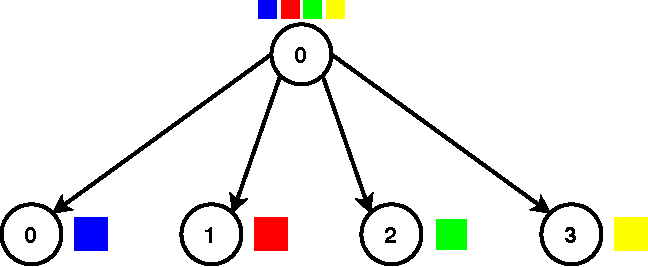
\includegraphics[width=0.9\columnwidth]{MPI_Scatter.pdf}
\centering
\caption{Illustration of Scatter Process}
\label{scatter}
\end{figure}

\begin{figure}[h!]
\centering
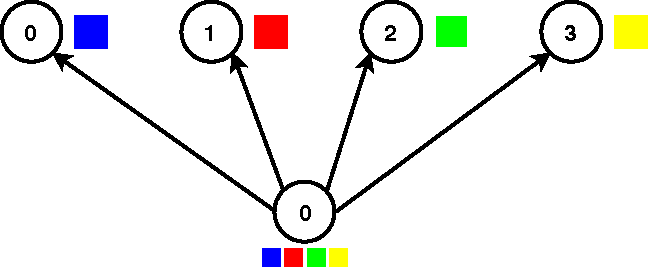
\includegraphics[width=0.9\columnwidth]{MPI_Gather.pdf}
\centering
\caption{Illustration of Gather Process}
\label{gather}
\end{figure}

\begin{figure}[h!]
\centering
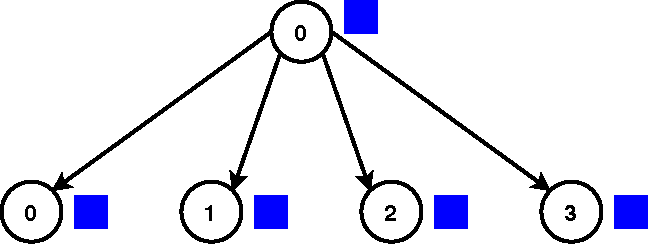
\includegraphics[width=0.9\columnwidth]{MPI_broadcast.pdf}
\centering
\caption{Illustration of broadcast Process}
\label{broadcast}
\end{figure}

\begin{figure}[h!]
\centering
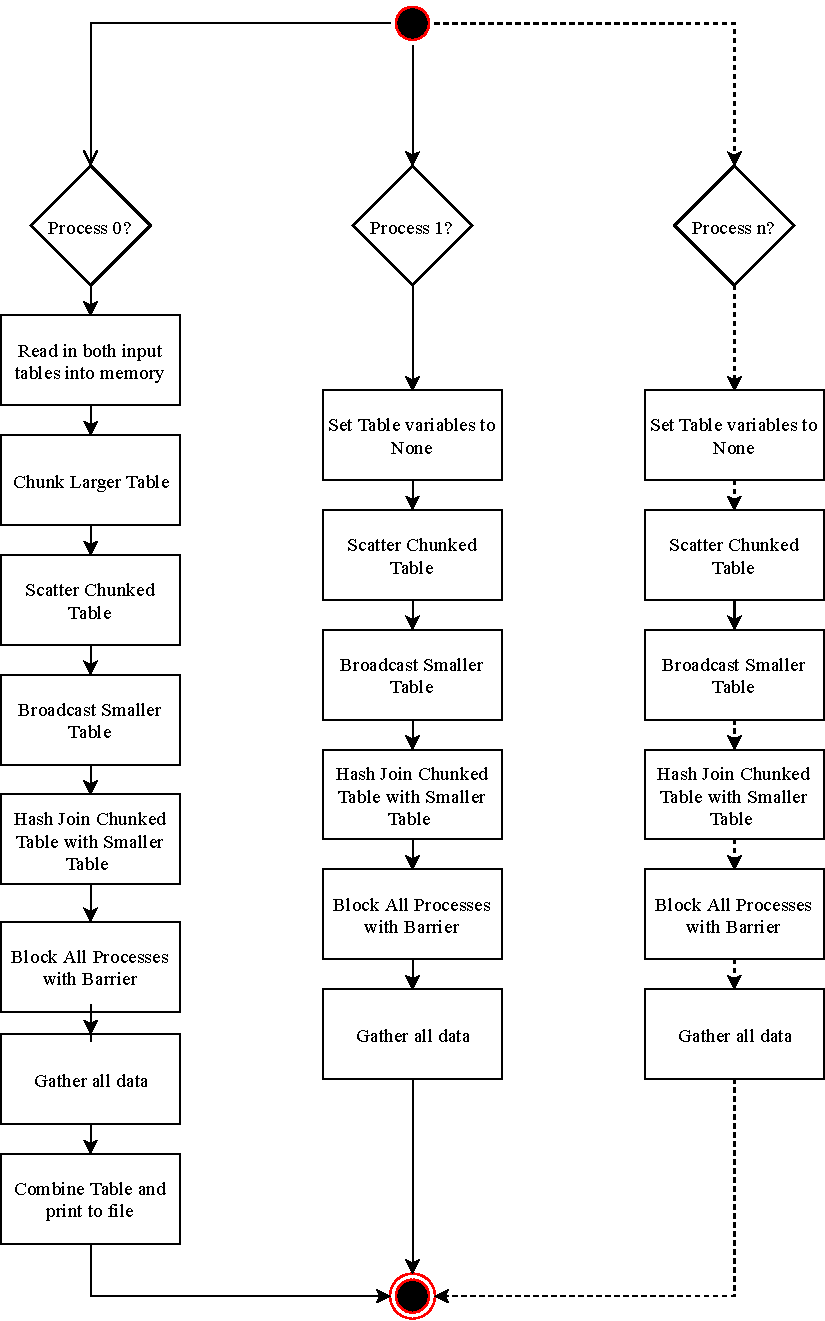
\includegraphics[width=\columnwidth]{FlowChar.pdf}
\centering
\caption{Flow Chart for MPI Collective Communication}
\label{flow}
\end{figure}

\subsubsection{Benchmark} 
Specific sections of code related to the master process are timed for benchmark purposes. The benchmark metrics include the time take to: read files into memory, scatter, broadcast, Barrier, send and receive. These results are were obtained on input files ranging between \num{10} - \num{100000000} rows and between \num{1} and \num{50} processes running on the cluster.

\section{Supplementary Utilities}
A selection of supplementary utilities were created, in addition to the aforementioned joining algorithms, to aid in the running and testing of each method. These utilities can be found within the \href{https://github.com/data-intensive-computing-4020/Project}{Github Repository}.

\subsection{Data Generation}
A Python script was created to produce sample data for the testing of the three algorithms. The output of this script is meant to simulate what real world data would look like from a traditional structured database. The data has been heavily simplified and only contains key information pertaining to the joining process, such as a key on which the join is performed and additional data to simulate other columns within the tables. The generator has two modes of operation,  realistic and worst case data sets.\\

The worst possible data set that could be generated is one where for every key in table one there is a corresponding key in table two. This proves to be the worst possible implementation for an inner join as there are no rows missed in the joining process. Moreover, both tables are the same size meaning that no minimisation can be achieved through hashing of the smaller table. Lastly, the keys in the two tables are generated in reverse order of each other, making the data inherently ordered backwards between the two tables.\\

The best case scenario of data generation aims to show a more realistic sample data set. Here, one table is created to have a one fifth the number of keys as the other table, minimising the total number of joins that need to be performed by five times.

\subsection{Verification of Results}
Another application was made that took in the results of the three scripts and compared the results of the joins to ensure that all three produced the correct outputs. This was done by reading in each table and then performing a sort on the rows as some algorithms produce differently ordered output results. Next, the results were checked for equality. If an error is found, then the user is informed accordingly. 

\subsection{Controller}
The controller application enables the tester to generate required sample data, run all three join algorithms as well as the result verifier with one command. Run time parameters enable the tester to specify the number of rows to generate, the number of nodes to run the MPI tests on, what algorithms they wish to run, and the kind of data (best case or worst case) to generate. The controller also informs the join scripts of what to name their join outputs and benchmark result files, based on the user input run time parameters.

\subsection{Benchmarker}
Lastly, a script was made to recursively call the controller, enabling a batch of benchmarks to be run over a range of array sizes and node counts. This application drastically reduces the total time taken to run tests on the system as many tests, in a multitude of configurations, can be run sequentially. 

\section{Experiment Environment}
The algorithms were all run on a cluster named Jaguar1 that contains \num{9} nodes. Each node has an Intel Core i7 950 CPU @ 3.07GHz. The cluster nodes have varying sizes of 12GB to 24GB memory with some nodes utilizing SSD and others HDD. The nodes compromise of 4 cores with 8 threads each, totalling 72 threads on the entire cluster. A machinefile is needed to specify the nodes to use in the execution of the code.\\

This set-up is not ideal as it makes no use of queueing, resulting in sharing cluster resources between different simultaneous program executions. This is contradictory to the assumption stated in Section X, which assumed that the cluster utilization would be uncontested during benchmarking. As a result, even though the benchmark results are accurate, they proved to be inconsistent between executions and are thus unreliable. The cluster experienced a number of issues related to storage space as it could not store the temporary files that were created during the execution of some algorithms. The cluster also suffered from instability and would break the connection pipe between users and the cluster with no reason. Another issue arose from the distribution of the MPI data as it would evenly distribute the workload between uneven nodes as they had different memory and disk drive specifications.  This resulted in faster nodes waiting for slower nodes to finish processing their data before they were broadcast, introducing a hardware overhead in the benchmark tests. 

\section{Results}
A wide selection of tests were performed on the each algorithm, totalling 1680 joined tables across the three algorithms. These tests were run with the aid of the benchmark utility, enabling a programmatic input of different sample sizes and node configurations to conduct each join. In total, close to 5 billion rows where join across all tables and algorithms. This section presents the results and in the following sections these results are discussed and analysed. All graphs generated are logarithmic in both axis, with different lines representing different join algorithm configurations, such as additional MPI processes.\\

Figure \ref{graph1} shows an average output of all three algorithms, with different colours representing different operation modes. Not all tested configurations are shown in this graph but rather key implementations such as increasing number of nodes.

\begin{figure*}[h!]
\centering
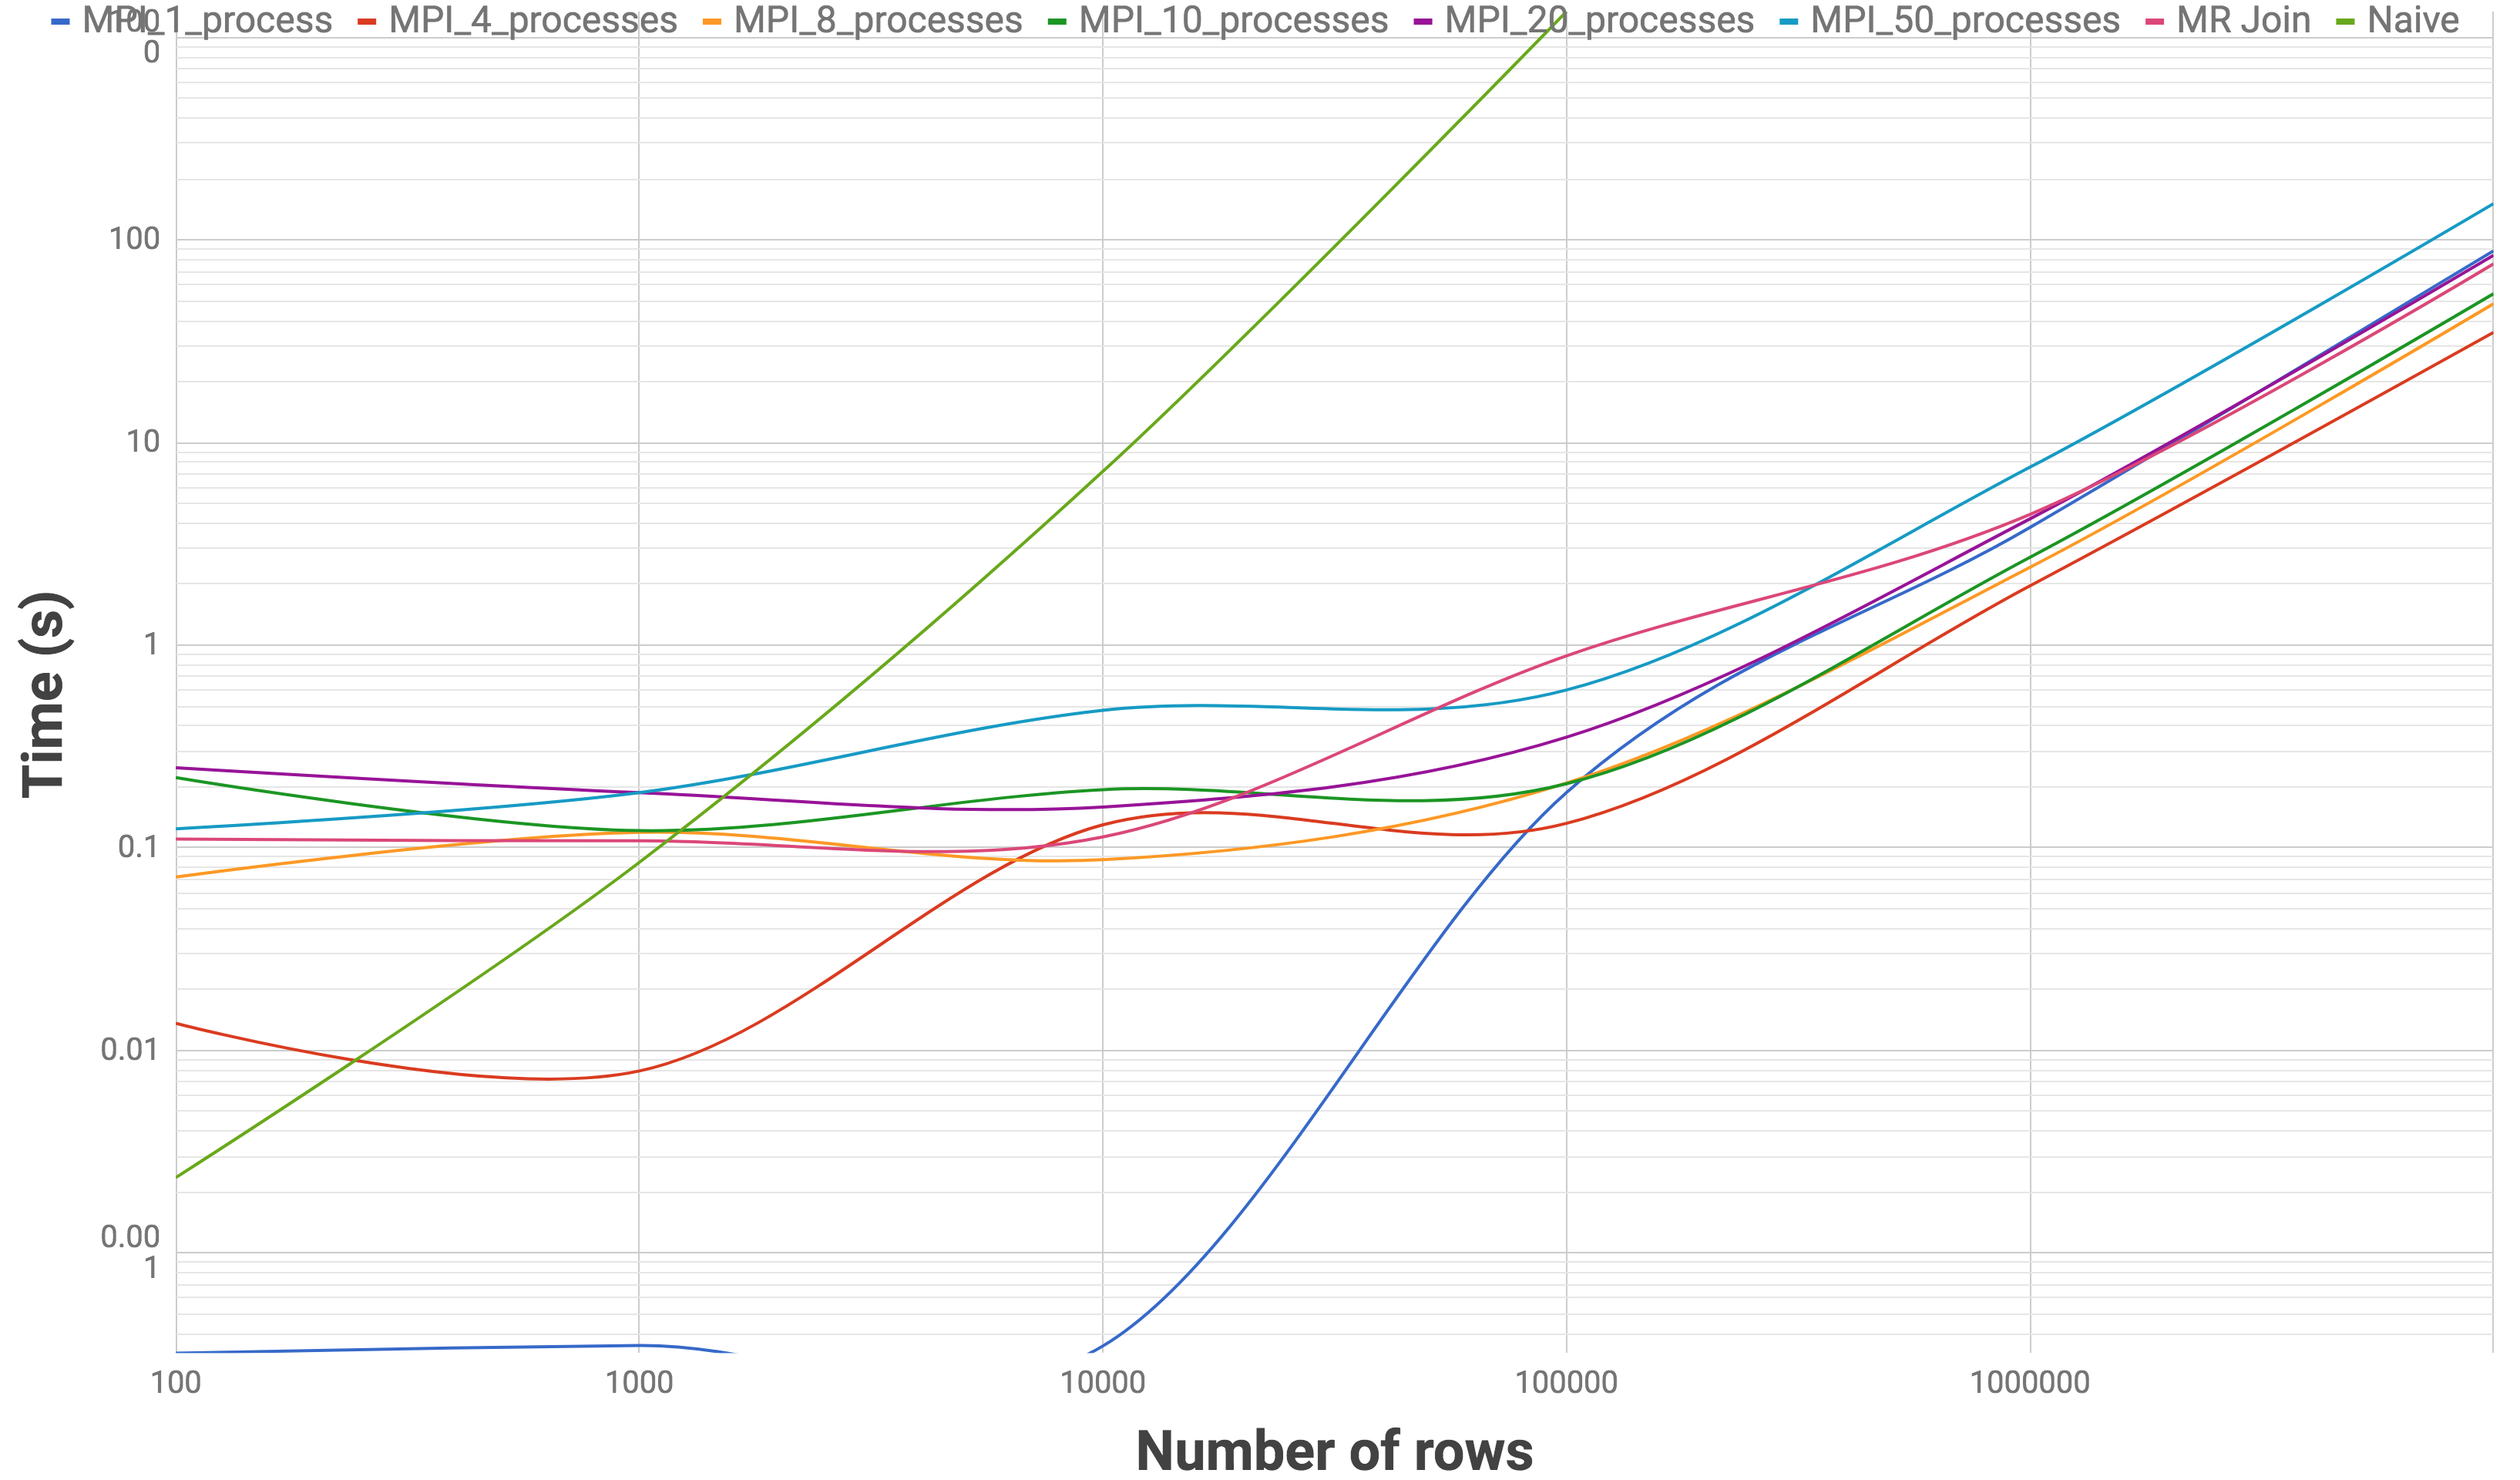
\includegraphics[width=\textwidth]{graph2.png}
\centering
\caption{Benchmark of All Join Algorithms over a Series of Row sizes}
\label{graph1}
\end{figure*}

Figure \ref{graph2} represents computation time of the different algorithms at a lower row counts.

\begin{figure*}[h!]
\centering
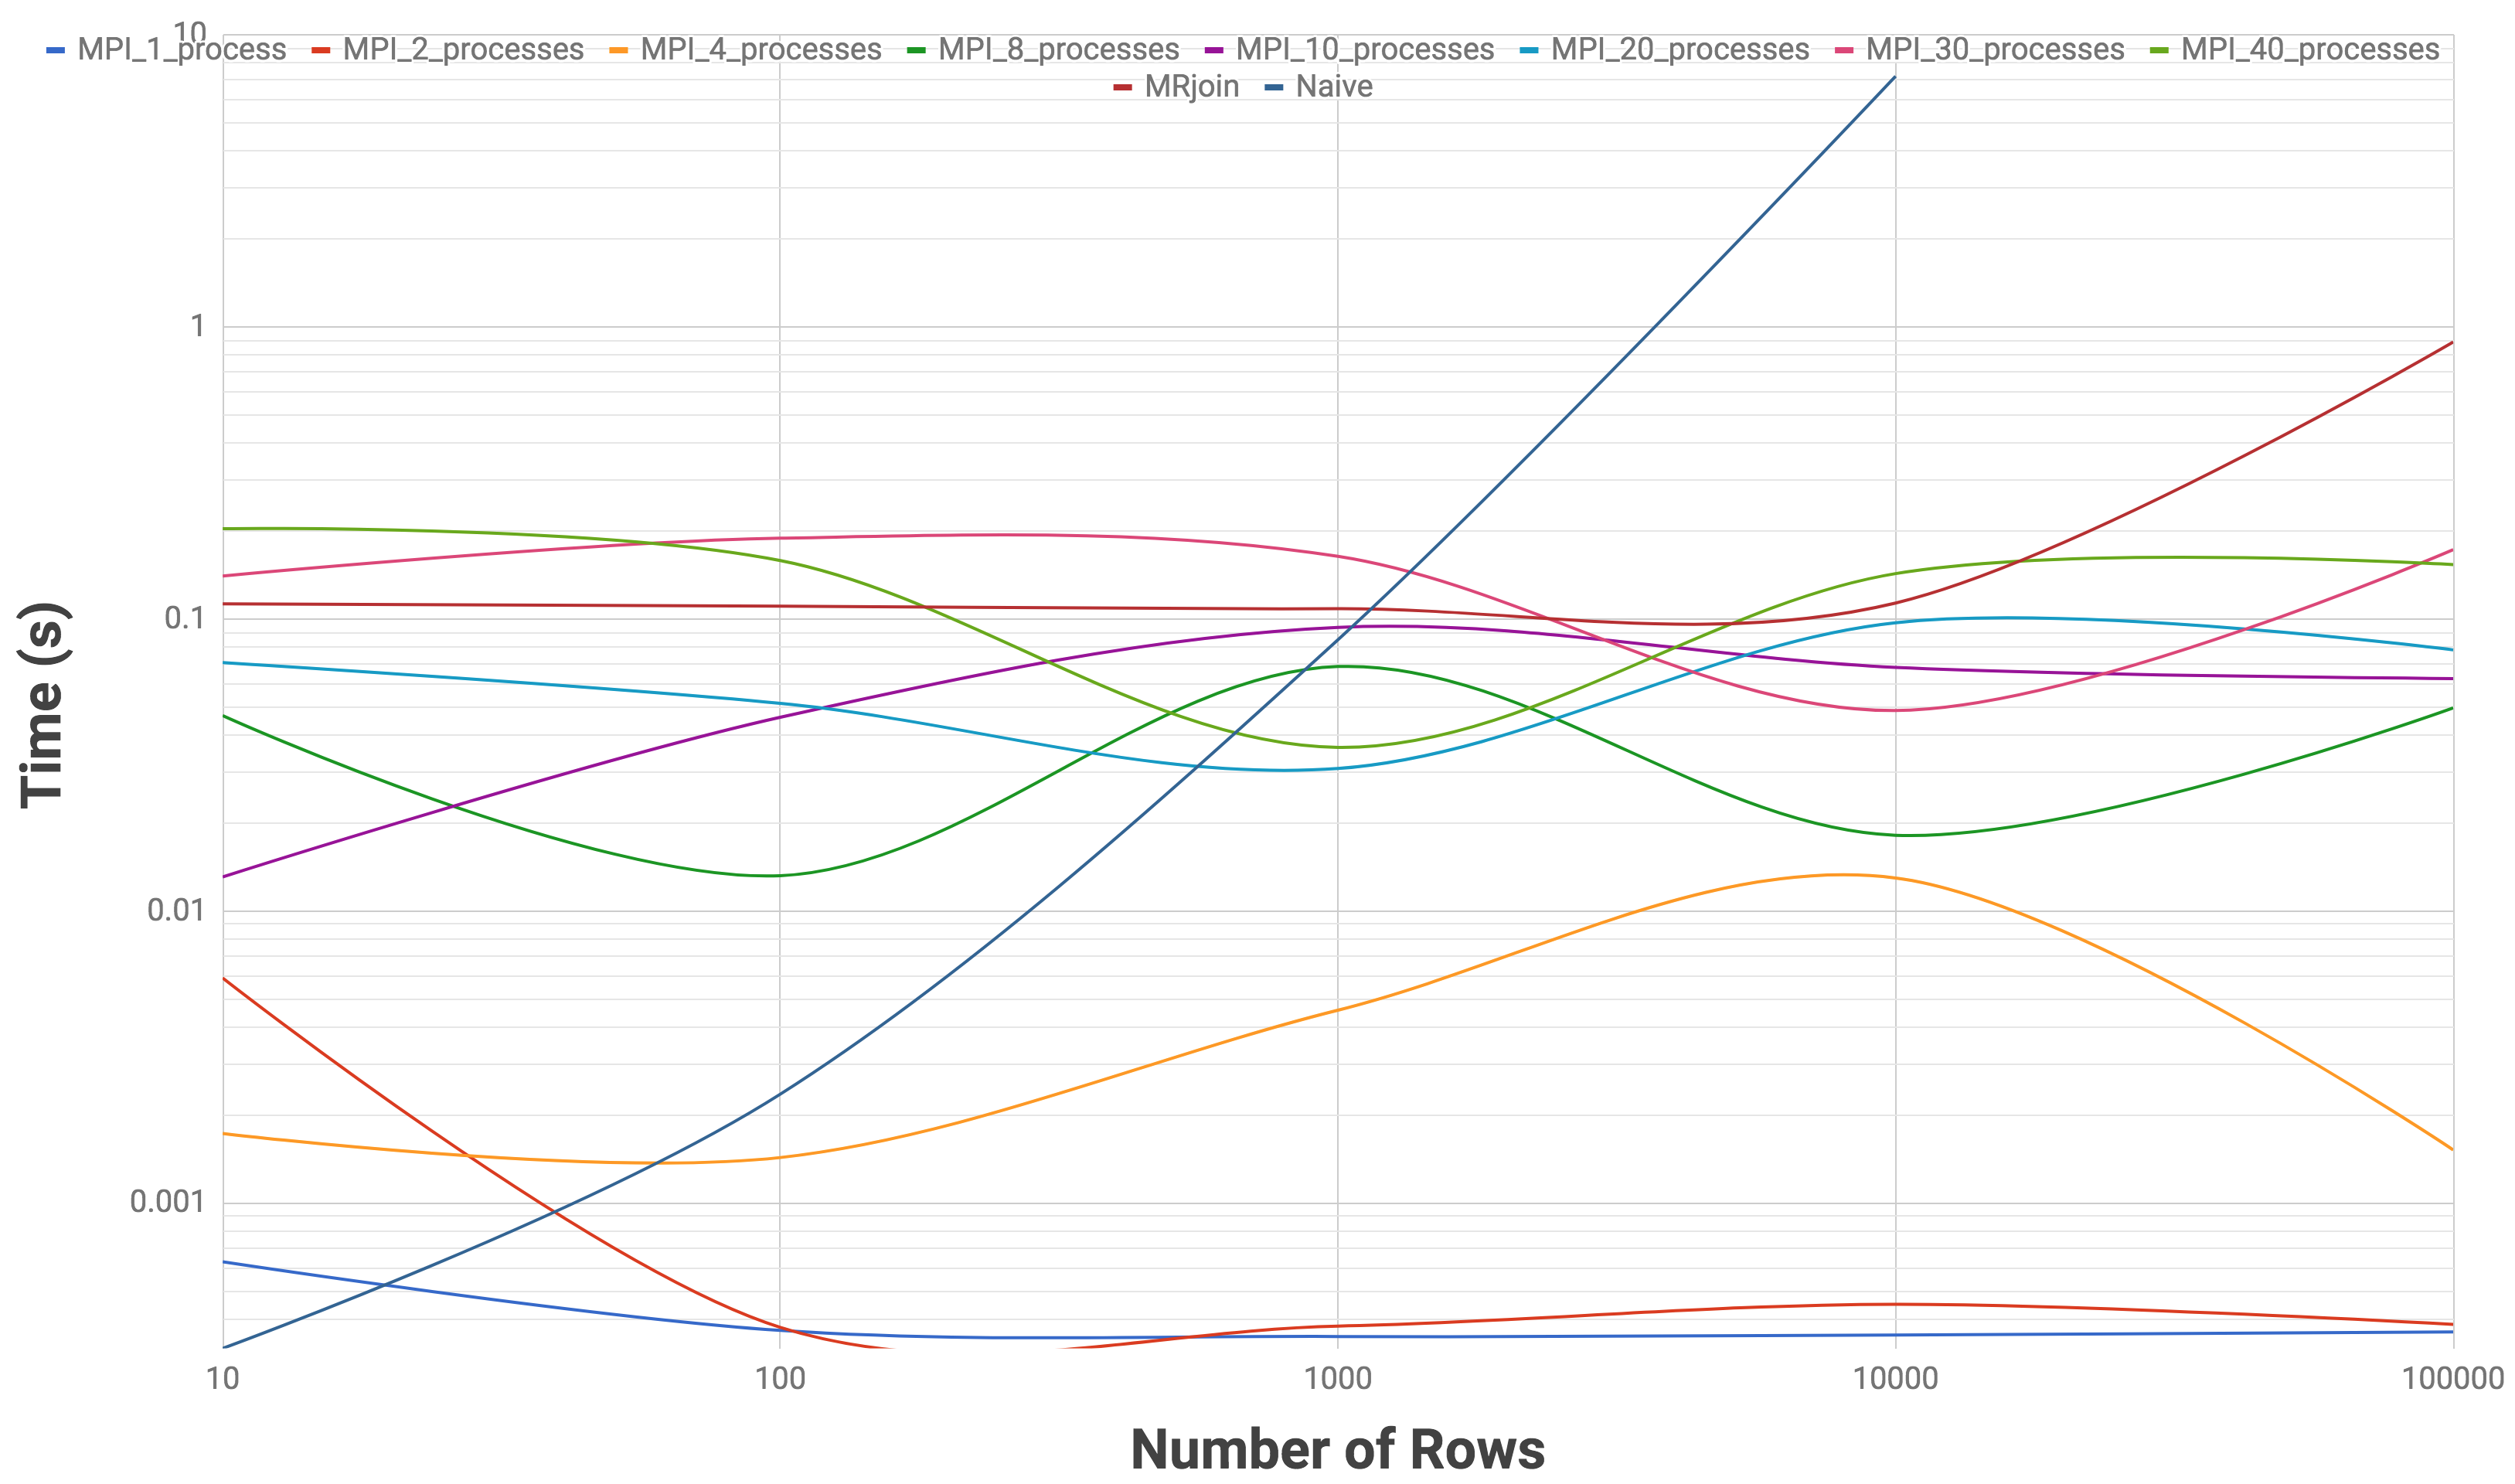
\includegraphics[width=\textwidth]{graph1.png}
\centering
\caption{Benchmark of Low Row Counts}
\label{graph2}
\end{figure*}

Figure \ref{graph3} shows the key testing information, used to invert the ideal algorithms for different sample sizes.

\begin{figure*}[h!]
\centering
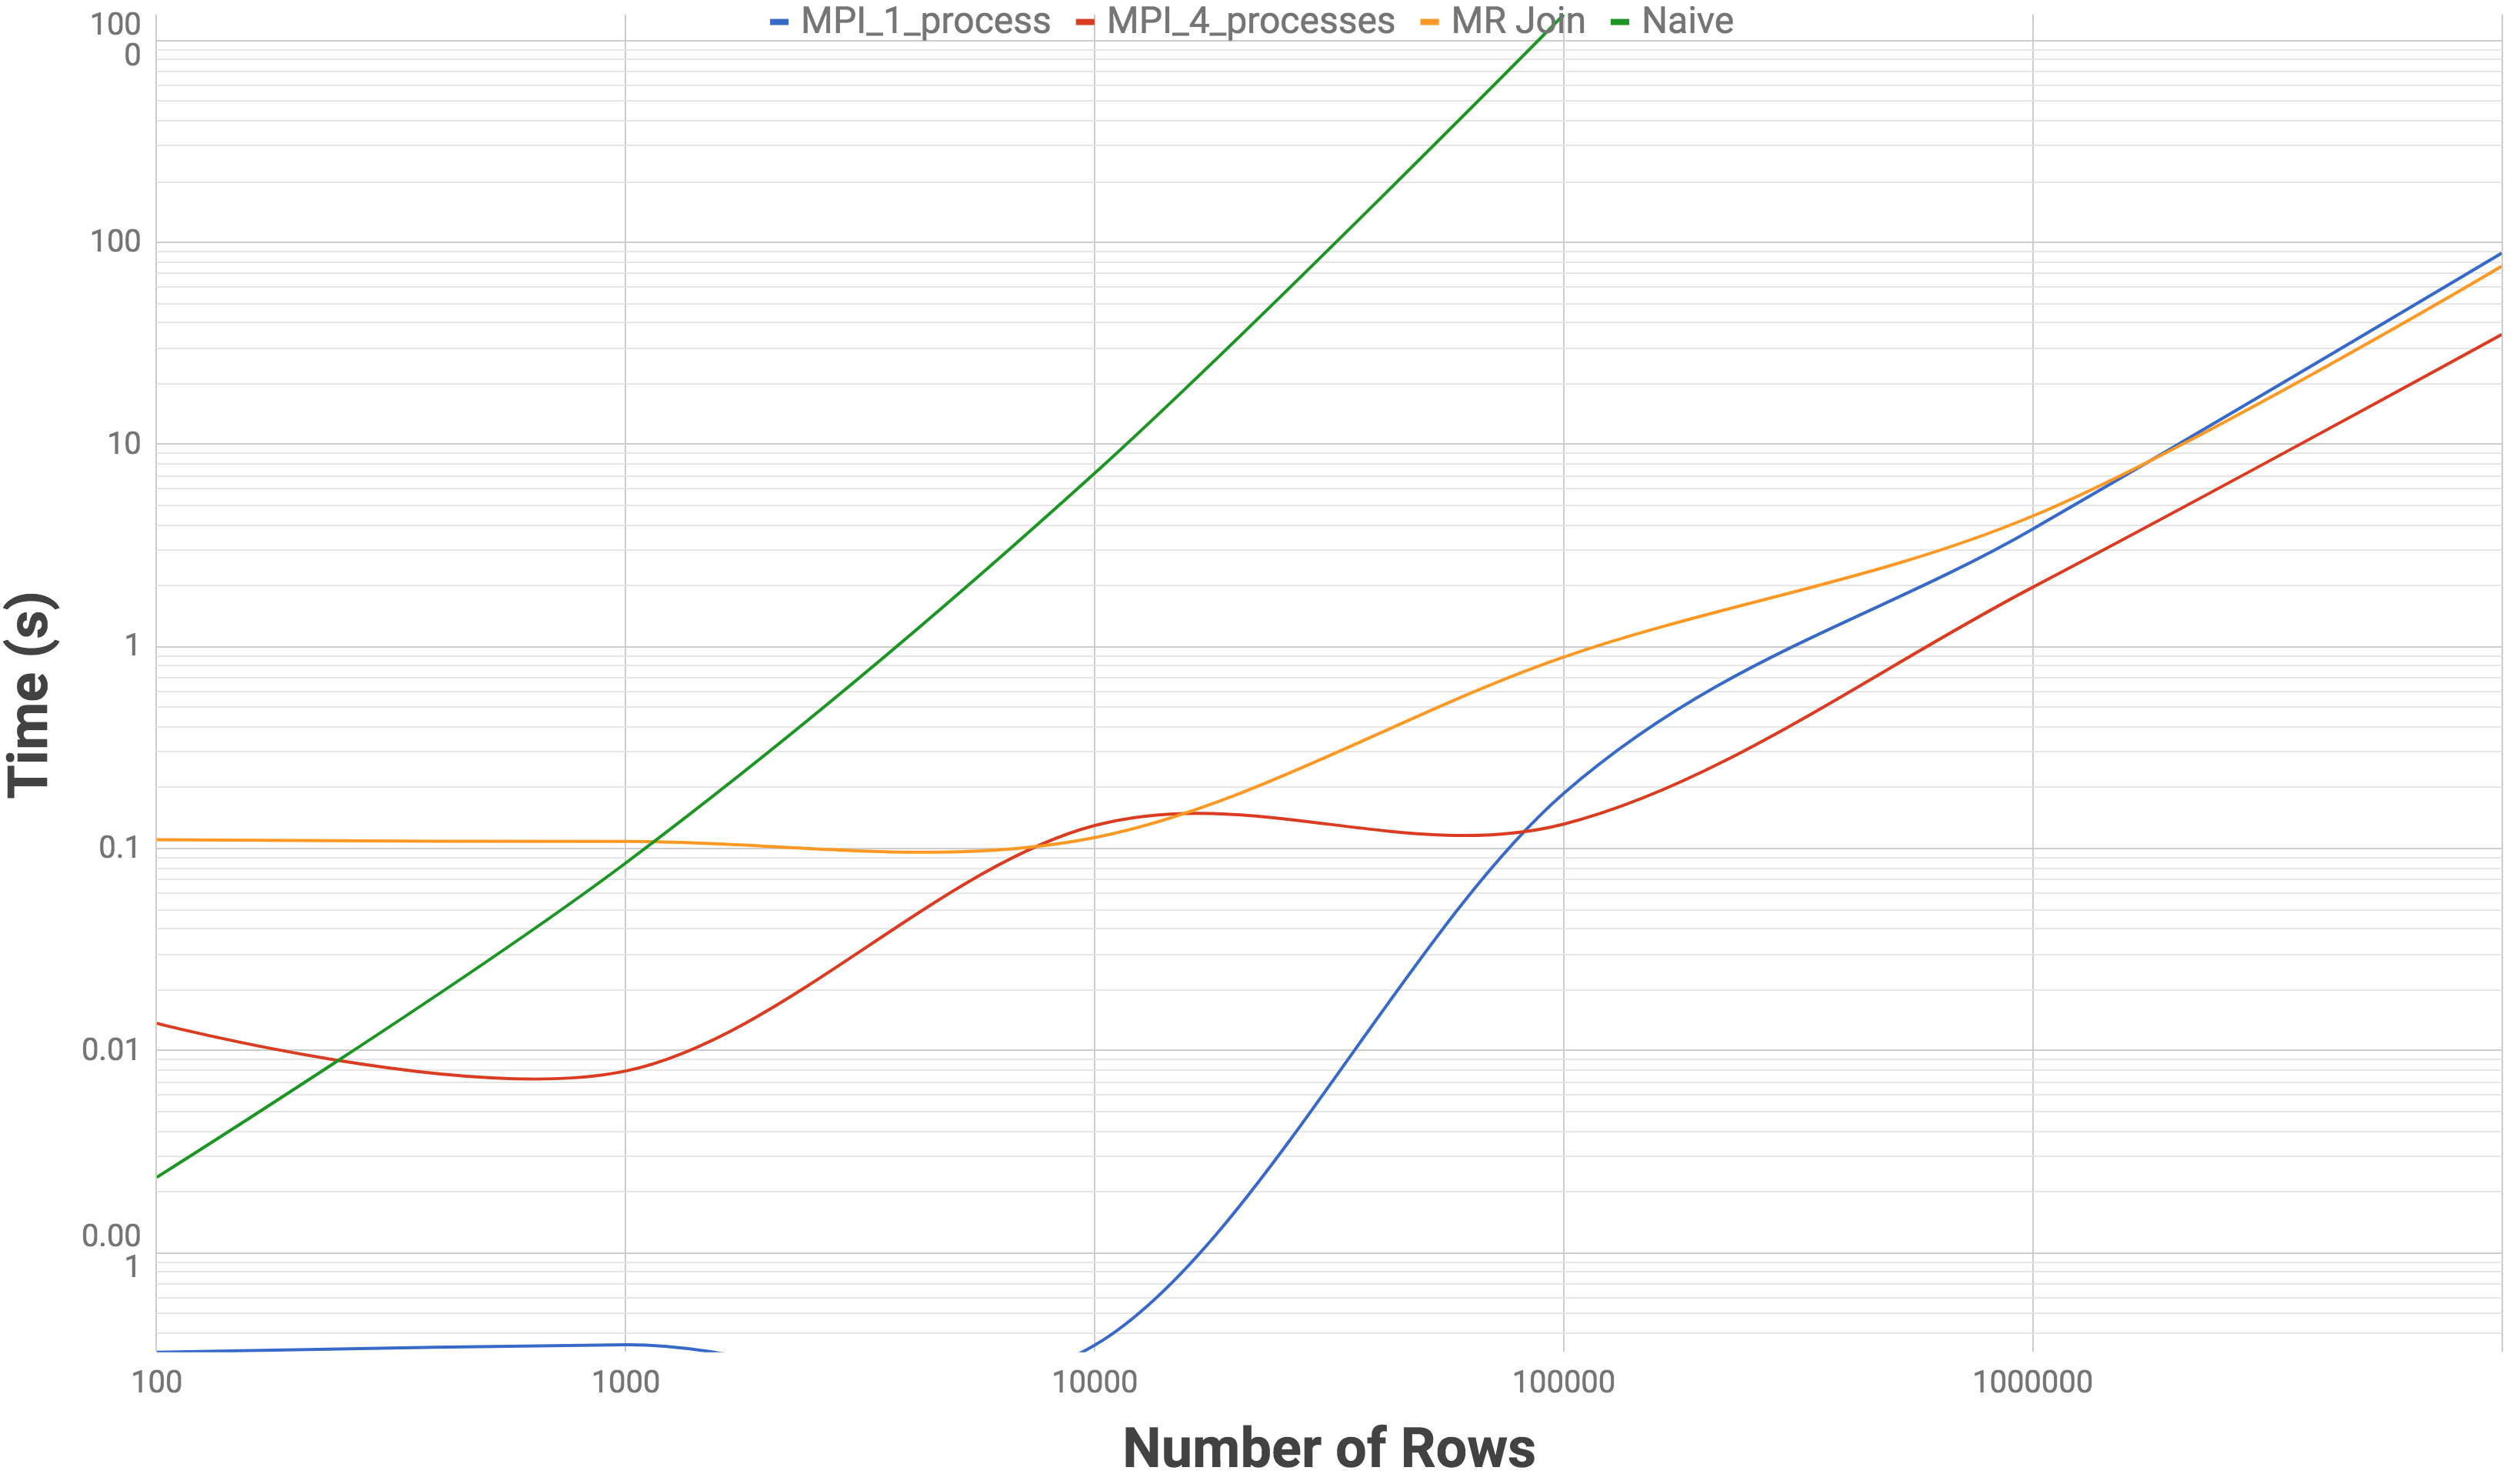
\includegraphics[width=\textwidth]{graph3.png}
\centering
\caption{Benchmark of Key Algorithm Implementations}
\label{graph3}
\end{figure*}

Testing results are analysed in the following section.

\section{Critical Analysis}

Each presented graph was chosen to highlight a specific trend present in the testing results. 

Reference \ref{graph1} shows the general trend of the algorithms, with the expected pattern of increasing computation time with increased row count. From this graph, it is clear that the best algorithm below a particular size of data set is MPI hash join running on one node. Over and above a particular size, this is no longer the case. This crossover point can be seen in Reference \ref{graph3}, clearly highlighting that above a sample size of 100,000 rows, MPI hash join running on one process is slower than MPI hash join running on 4 processes. This graph only shows MPI with one and four nodes as these were the best results obtained from all cluster configurations run.\\

Reference \ref{graph2} shows that at low row counts, there is no clear trend with increased row number but rather that the number of processes results in slower computation with the MPI implementation. This behaviour is as a result of the added overhead associated with additional MPI processes. The network distribution time far outweighs the added computation power from spreading the information over a cluster at these low row counts. The network I/O is simply much higher than the time complexity of conducting the join.\\

All three graphs show the naive solution quickly ramping up and out of the range of the other implementation. This behaviour is expected due to the squared time complexity of the algorithm. With that said, figure \ref{graph2} shows that below 20 rows in the table, the naive solution proves to be the fastest joining algorithm, as was predicted in the algorithm discussion section of this paper.\\

The MapReduce join is never the fastest solution in any test. This is due to the overhead associated with the algorithm, primary the creation and deletion of temporary files. Figure 3 shows that above a 2 million rows, the map reduce implementation is faster than the single process MPI implementation. Despite this, it is still slower than the MPI four processor implementation. 

\subsection{Selection of Optimum Algorithm}
These results show that there is no single possible best solution for all input data types and sizes. A hybrid approach is therefore proposed wherein different algorithms are utilized based on the input sample data. If the sample data is below 20 rows, then the nested for loop join is recommended. For joins between 20 and 100 000 rows, a single MPI implementation hash join is recommended. For this sample size, there is no benefit in using the MPI framework and a standard hash join would outperform these results as it would not have the associated library overhead. For sample size over 100 000 rows, MPI shows increased performance, with a four process implementation beating the single process result. \\

Tests were only conducted up to 10 000 000 rows but over an above this the trend will continue, meaning the success criteria that scaling computational resources result in faster join times was met. Thus, there will be a threshold in higher row counts where more than four MPI nodes will achieve faster performance but benchmarks of datasets up to this size were not conducted in this paper due to the required computational resources required to conduct tests of this size.

\subsection{Justification for MPI Scaling Results}
The MPI join algorithm performance showed a number of interesting results, some of which are contradictory to what one would expect. For example, it was expected that the total time of the join algorithm would drop with added computational power allocated to the join. This trend was observed only between one MPI process and four MPI processes, above a specific table size. This indicates that the network overhead associated with the MPI implementation outweighs the gained speed from additional computation power. Additionally there is an inherent overhead resulting from how Mpi4py transmits information between processes. All Python objects are first pickled before being sent, resulting in heavy network overhead. These results will differ if C was used, for example, as this does not require the pickling of objects before transmission and unpickling after being received\cite{TutorialsPoint2018}.\\

The MPI join algorithm running on one process was shown to be the fastest implementation below a threshold as this is effectively the standard hash join algorithm implemented in python. There is no network overhead due to MPI for this as no transmission between processes is required.

\subsection{Future Improvements}
The advantages of MapReduce used in combination with a Hadoop cluster are never leveraged to compare the processing performance of this architecture to MPI. This would surpass the serially implemented MapReduce through the use of a parallelized MapReduce. MapReduce with Hadoop should be implemented and benchmarked for a more comparative analysis with MPI.  

\section{Conclusion}
This paper presented a comparison between different table join algorithms, implemented in Python. The algorithms were discussed in detailed and then benchmarked. This showed that a distributed, cluster based algorithm, implemented with MPI, outperformed a parallel algorithm, created with MapReduce. The results were critically analysed, finding justification for performance of each algorithm. Future improvements were then proposed, providing recommendations as to future work.  

%\vfill\null
\newpage
\bibliographystyle{IEEEtran}
\bibliography{Mendeley.bib}

\end{document}